\begin{frame}{A 3 page book}

\begin{columns}[T,onlytextwidth]
	\begin{column}{0.5\textwidth}
		\centering
        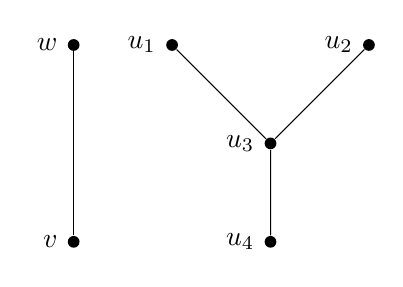
\begin{tikzpicture}[scale=2.5]
            \node[circle, fill, inner sep=1.5pt, label=left:\(v\)] (v) at (0,0) {};
            \node[circle, fill, inner sep=1.5pt, label=left:\(w\)] (w) at (0,1) {};
            \draw (v) -- (w);

            \node[circle, fill, inner sep=1.5pt, label=left:\(u_1\)] (u1) at (0.5, 1) {};
            \node[circle, fill, inner sep=1.5pt, label=left:\(u_2\)] (u2) at (1.5, 1) {};
            \node[circle, fill, inner sep=1.5pt, label=left:\(u_3\)] (u3) at (1, .5) {};
            \node[circle, fill, inner sep=1.5pt, label=left:\(u_4\)] (u4) at (1, 0) {};
            \draw (u1) -- (u3);
            \draw (u2) -- (u3);
            \draw (u3) -- (u4);
        \end{tikzpicture}
			
		\scriptsize \(\Gamma = K_2 \cup K_{1,3}\) 
        
        i.e. \(\Gamma\) is an edge and the ``\(Y\)-graph''.
	\end{column}

	\begin{column}{0.5\textwidth}
		\centering
        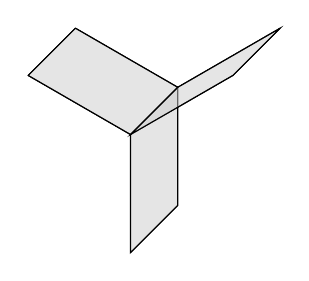
\begin{tikzpicture}[
            scale=1.5,
            x={(1cm,0cm)},
            y={(0cm,1cm)},
            z={(0.4cm,0.4cm)}
        ]

        \coordinate (vu3) at (0, 0, 0);
        \coordinate (wu3) at (0, 0, 1);
        
        \coordinate (vu1) at (-.866, .5, 0);
        \coordinate (vu2) at (0, -1, 0);
        \coordinate (vu4) at (.866, .5, 0);

        \coordinate (wu1) at (-.866, .5, 1);
        \coordinate (wu2) at (0, -1, 1);
        \coordinate (wu4) at (.866, .5, 1);



        % spine
        \draw (vu3) -- (wu3);

        % pages
        \draw (vu3) -- (vu1);
        \draw (vu3) -- (vu2);
        \draw (vu3) -- (vu4);

        \draw (wu3) -- (wu1);
        \draw (wu3) -- (wu2);
        \draw (wu3) -- (wu4);

        \draw (vu1) -- (wu1);
        \draw (vu2) -- (wu2);
        \draw (vu4) -- (wu4);

        % fill in pages as 3D quadrilaterals (one per page) and draw their outlines
        \filldraw[fill=gray!40, fill opacity=0.5, draw=black] (vu3) -- (vu1) -- (wu1) -- (wu3) -- cycle;
        \filldraw[fill=gray!40, fill opacity=0.5, draw=black] (vu3) -- (vu2) -- (wu2) -- (wu3) -- cycle;
        \filldraw[fill=gray!40, fill opacity=0.5, draw=black] (vu3) -- (vu4) -- (wu4) -- (wu3) -- cycle;

        \end{tikzpicture}

		\scriptsize A book is a connected component of \(\Conf_2(\Gamma)\).
    \end{column}
\end{columns}

\end{frame}